\documentclass[tikz,border=4pt]{standalone}
\usepackage{amsmath,amssymb}
\usetikzlibrary{arrows.meta}
\definecolor{navy}{HTML}{17365D}
\definecolor{xaxis}{HTML}{B6252D}
\definecolor{yaxis}{HTML}{217A3C}
\definecolor{zaxis}{HTML}{215AAB}
% One continuous opaque gripper body, with no drawn internal edge lines.
% Fingers remain downward. A further positive yaw makes its open face look right.
% R_z(110 deg) is illustrative geometry, not an experimental angle.
\newcommand{\PoseGripper}{%
  \pgfmathsetmacro{\GripYaw}{110}
  \pgfmathsetmacro{\GripXX}{cos(\GripYaw)-0.55*sin(\GripYaw)}
  \pgfmathsetmacro{\GripXY}{-0.42*sin(\GripYaw)}
  \pgfmathsetmacro{\GripYX}{-sin(\GripYaw)-0.55*cos(\GripYaw)}
  \pgfmathsetmacro{\GripYY}{-0.42*cos(\GripYaw)}
  \begin{scope}[x={(\GripXX cm,\GripXY cm)},
    y={(\GripYX cm,\GripYY cm)},z={(0cm,1cm)}]
    % Visible side faces of the same extruded body; flat fills without strokes.
    \path[fill=black!42]
      (-0.23,-0.14,-0.38)--(-0.23,0.14,-0.38)
      --(-0.23,0.14,0.48)--(-0.23,-0.14,0.48)--cycle;
    \path[fill=black!42]
      (0.42,-0.14,-0.38)--(0.42,0.14,-0.38)
      --(0.42,0.14,0.90)--(0.42,-0.14,0.90)--cycle;
    \path[fill=black!12]
      (0.42,-0.14,0.90)--(0.42,0.14,0.90)
      --(0.16,0.14,0.90)--(0.16,-0.14,0.90)--cycle;
    \path[fill=black!42]
      (0.16,-0.14,0.90)--(0.16,0.14,0.90)
      --(0.16,0.14,1.13)--(0.16,-0.14,1.13)--cycle;
    \path[fill=black!12]
      (0.16,-0.14,1.13)--(0.16,0.14,1.13)
      --(-0.16,0.14,1.13)--(-0.16,-0.14,1.13)--cycle;
    \path[fill=black!12]
      (-0.16,-0.14,0.90)--(-0.16,0.14,0.90)
      --(-0.42,0.14,0.90)--(-0.42,-0.14,0.90)--cycle;
    % A single filled contour joins both fingers, palm and wrist.
    \path[fill=black!27]
      (-0.42,-0.14,-0.38)--(-0.23,-0.14,-0.38)
      --(-0.23,-0.14,0.48)--(0.23,-0.14,0.48)
      --(0.23,-0.14,-0.38)--(0.42,-0.14,-0.38)
      --(0.42,-0.14,0.90)--(0.16,-0.14,0.90)
      --(0.16,-0.14,1.13)--(-0.16,-0.14,1.13)
      --(-0.16,-0.14,0.90)--(-0.42,-0.14,0.90)--cycle;
  \end{scope}
}

\begin{document}
% Schematic pose coordinates; no experimental dimensions or measurements.
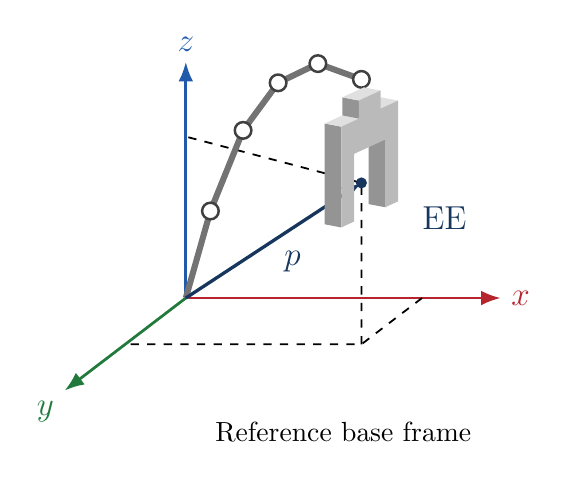
\begin{tikzpicture}[x={(1cm,0cm)},y={(-0.55cm,-0.42cm)},z={(0cm,1cm)},
 font=\large,axis/.style={-{Latex[length=2.5mm]},line width=1pt},
 projection/.style={black,dashed,line width=0.65pt}]

\coordinate (O) at (0,0,0);
\coordinate (P) at (3,1.4,2.05);
\draw[axis,xaxis] (O)--(4,0,0) node[right] {$x$};
\draw[axis,yaxis] (O)--(0,2.8,0) node[below left] {$y$};
\draw[axis,zaxis] (O)--(0,0,3) node[above] {$z$};
\draw[projection] (3,0,0)--(3,1.4,0)--(0,1.4,0);
\draw[projection] (3,1.4,0)--(P)--(0,0,2.05);
% Illustrative joint chain from the base origin to the gripper wrist. The link
% inclinations fan out steadily -- roughly 74, 68, 54 and 26 degrees above the
% horizontal -- so the chain leaves the origin between the z axis and the
% position vector, flattens over the top and drops onto the wrist at about 20
% degrees below the horizontal, where the last circle rests tangentially on the
% gripper. No joint circle is drawn at the origin, so the base frame stays
% visible, and every circle clears the axes, the vector p and the projections.
\coordinate (J0) at (0,0,0);
\coordinate (J1) at (0.45,0.25,1.21);
\coordinate (J2) at (1.03,0.55,2.36);
\coordinate (J3) at (1.64,0.85,3.09);
\coordinate (J4) at (2.31,1.15,3.46);
\coordinate (J5) at (3.00,1.40,3.365);
\draw[black!55,line width=2.2pt,line cap=butt,line join=round]
  (J0)--(J1)--(J2)--(J3)--(J4)--(J5);
\draw[axis,navy,line width=1.2pt] (O)--(P) node[midway,below right] {$p$};
\foreach \joint in {J1,J2,J3,J4,J5}{
  \filldraw[fill=white,draw=black!75,line width=0.9pt]
    (\joint) circle (3.0pt);
}
\begin{scope}[shift={(P)}]
  \PoseGripper
\end{scope}
\fill[navy] (P) circle (2.0pt);
\node[anchor=west,navy] at (3.65,1.4,1.60) {EE};
\node[anchor=north west,font=\normalsize] at (0.25,0,-1.45) {Reference base frame};
\end{tikzpicture}
\end{document}
